\documentclass{beamer}
\usetheme{default}
\setbeamertemplate{navigation symbols}{}
%	
\usepackage{subfig}
\usepackage{amsmath, amsthm, amssymb}
\usepackage{float}
\usepackage{rotating}
\usepackage{graphicx}
\usepackage{longtable}
\usepackage{xcolor}
\usepackage{bm}
\usepackage{tikz}
\usetikzlibrary{shapes}
\tikzset{My Arrow Style/.style={single arrow, fill=red!50, anchor=base, align=center,text width=.5cm,rotate =270}}
\newcommand{\MyArrow}[2][]{\tikz[baseline] \node [My Arrow Style,#1] {#2};}
\tikzset{My 2Arrow Style/.style={single arrow, fill=red!50, anchor=base, align=center,text width=.5cm,rotate =90}}
\newcommand{\MyArrowUp}[2][]{\tikz[baseline] \node [My 2Arrow Style,#1] {#2};}
%\newcommand{at}{\begin{matrix}}
%\newcommand{\emat}{\end{matrix}}
\newcommand{\EE}{\mathbb E}

\newtheorem{acknowledgement}[theorem]{Acknowledgement}
\newtheorem{algorithm}[theorem]{Algorithm}
\newtheorem{assumption}{Assumption}
\newtheorem{axiom}{Axiom}
\newtheorem{case}[theorem]{Case}
\newtheorem{claim}[theorem]{Claim}
\newtheorem{conclusion}[theorem]{Conclusion}
\newtheorem{condition}[theorem]{Condition}
\newtheorem{conjecture}{Conjecture}
\newtheorem{criterion}[theorem]{Criterion}
\newtheorem{proposition}{Proposition}
\newtheorem{summary}[theorem]{Summary}
\newtheorem{exercise}{Exercise}
\newtheorem{notation}{Notation}
\newtheorem{remark}{Remark}
%\graphicspath{{graphs//}}

\title {Optimal fiscal policy with incomplete asset markets}
\author{Anmol Bhandari, David Evans, Mikhail Golosov, Thomas J. Sargent}

\date{October 2013}
% \today will show current date.
% Alternatively, you can specify a date.
%
\begin{document}
%
\begin{frame}
\titlepage

\end{frame}
\section{Introduction}
\subsection{}
\begin{frame}
\frametitle{Optimal taxation under commitment and a representative agent}

\begin{itemize}

 \item \textbf{Incomplete markets}

 \quad \color{red}$\rightarrow$ \color{black} assets with alternative exogenous payoff patterns

 \item \textbf{Linear tax schedules}

 \quad \color{red}$\rightarrow$ \color{black}Proportional tax on labor earnings (maybe  {\em nonnegative} transfers)

 \item \textbf{Aggregate shocks}

 \quad \color{red}$\rightarrow$ \color{black} To productivities, government expenditures,  etc.

 \end{itemize}
\end{frame}



\begin{frame}
\frametitle{Questions}

\begin{enumerate}
\item \textbf{Tax rate}: How should  government accumulate or decumulate assets to smooth tax  distortions
\item \textbf{Government debt}: Why do different governments issue different amounts of debt?
Difference answers under polar assumptions:  LS -- complete markets; AMSS --- a risk-free bond only
\begin{itemize}
 \item [+] Lucas Stokey (1984): Inherited from initial condition
 \item [+ ] AMSS (2002): Govt. accumulates assets sufficient to finance activities using interest revenues
\end{itemize}

\end{enumerate}
\end{frame}


\begin{frame}
\frametitle{Our analysis}

\begin{enumerate}
\item \textbf{Asset structure}
\begin{itemize}
\item [+] We restrict government  to trade a single asset only
\item [+] We exogenously restrict asset payoffs

 $\Longrightarrow$ E.g., bonds that pay less during adverse times

 \end{itemize}
\item \textbf{Forces}
\begin{itemize}
\item Asset {\color{black} \textbf{levels} } can help smooth tax distortions {\color{black} \textbf{ across  states}}
\item This differs from the  role of debt in previous incomplete markets  economies where { \color{black} \textbf{changes}} in debt levels help smooth tax distortions {\color{black}  \textbf{ over  time}}
\end{itemize}
\end{enumerate}

\end{frame}


\section{Environment}
\subsection{}

\begin{frame}
 \frametitle{Environment}
 \begin{itemize}
 \item \textbf{Uncertainty}: Markov aggregate shocks $s_t\in \mathcal{S}$
  \item \textbf{Demography}: Infinitely lived representative agent plus a benevolent planner
  \item \textbf{Preferences }(Households)
  \begin{equation*}
\mathbb{E}_{0}\sum_{t=0}^{\infty } \beta^t  U\left(
c(s^t),l(s^t)\right)  \label{utility lifetime}
\end{equation*}%
  \item \textbf{Technology}: Aggregate output  $y_t=\theta_{t} l_{t}$
   \end{itemize}

\end{frame}

\begin{frame}
 \frametitle{Environment, II}
 \begin{itemize}
\item \textbf{Asset markets}: 
\begin{itemize}
 \item The government trades are restricted to an single asset
\item The payoff of a unit of government debt is given by a matrix $p_t$ parameterized by a $|\mathcal{S}|^2$ matrix $\mathbb{P}$
\[p_t=\mathbb{P}(s_{t}|s_{t-1})\]
\end{itemize}



  \item \textbf{Linear Taxes}: Agent $i$'s tax bill
\[- T_t + \tau_t \theta_{t}l_{t},  \ T_t \geq 0 \]

\item[]
  \item \textbf{Budget constraints} Let $q_t$ be the price of the asset,
  
  \begin{itemize}
   \item Agents: $ c_{t}+q_tb_{t}=\left( 1-\tau _{t}\right) \theta _{t}l_{t}+p_{t}b_{t-1}+T_{t},$ % \ T_t \geq 0$
  \item Government: $g_{t}+q_tB_{t}+T_t=\tau _{t}\theta_{t}l_{t}+p_{t}B_{t-1}, $% \ T_t \geq 0$
  \end{itemize}

\item[]
  \item \textbf{Market Clearing}
  \begin{itemize}
   \item Goods: $c_{t}+g_t = \theta _{t} l_{t}$

   \item Assets: $b_{t}+B_{t}=0$
\end{itemize}
  \item[]

\item \textbf{Initial conditions}: Assets $b_{-1}, B_{-1}$ and  $s_{-1}$
\end{itemize}

\end{frame}


\begin{frame}
 \frametitle{Ramsey Problem}

\begin{definition}
\textbf{Allocation, price system, government policy}

\end{definition}

\begin{definition}
\textbf{Competitive equilibrium}: Given $\left(b_{-1},B_{-1},s_{-1}\right) $ and $\left\{ \tau _{t},T_{t}\right\} _{t=0}^{\infty }$,
all allocations are individually rational, markets clear \footnote{Usually, we impose only  ``natural'' debt limits. }
\end{definition}

\begin{definition}
\textbf{Optimal competitive equilibrium}: A welfare-maximizing competitive
equilibrium for a given $\left( b_{-1},B_{-1},s_{-1}\right) $
\end{definition}

 \end{frame}

\begin{frame}
  \frametitle{Ramsey problem}
  
  \begin{enumerate}
  \item \textbf{Primal approach}: To eliminate tax rates and prices, use  consumer's first order conditions
  \item \textbf{Implementability constraints}:  Derive by iterating the consumer's budget equation forward  at every history

  $\Rightarrow$With incomplete market economies these impose  \emph{measurability restrictions} on Ramsey allocations

  \item  \textbf{Transfers: } We temporarily restrict transfers $T_t = 0$  $\forall t$. This is convenient for our analytical results.  We eventually show  that this assumption is not restrictive.

  \end{enumerate}


  \end{frame}

 \begin{frame}
 \frametitle{Sequential Ramsey problem}
\begin{equation*}
\max_{\{c_t,l_t,b_t\}} \EE_0\sum_{t=0}^\infty \beta^t U(c_t,l_t)
 \end{equation*}
 subject to

 \vspace{3mm}

 (a) \textbf{Feasibility}
\begin{subequations}
\begin{equation*}
c_t + g_t = \theta_t l_t
 \end{equation*}

(b) \textbf{Implementability constraints}

 \begin{equation*}
 \frac{b_{t-1}U_{c,t-1}}{\beta} = \frac{\EE_{t-1} p_t U_{c,t}}{p_t U_{c,t}}\EE_t\sum_{j=0}^\infty\beta^j\left( U_{c,t+j}c_{t+j}+U_{l,t+j}l_{t+j}\right)\text{  for $t\geq 1$ }
 \end{equation*}
\begin{equation*}
b_{-1} = \frac1{U_{c,0}}\EE_0\sum_{t=0}^\infty \beta^t\left(U_{c,t}c_t+U_{l,t}l_t\right)
 \end{equation*}
\end{subequations}
  \end{frame}

 
\begin{frame}
\frametitle{Roadmap, the questions}
 
	\begin{enumerate}
	\item The properties of the optimal allocation  are a function of \textbf{returns on the debt}
	\begin{itemize}
	 \item Prices: $\{q_t(s^t|B_{-1},s_{-1})\}_t$
	 \item Payoffs: $\mathbb{P}$
	\end{itemize}
	
\emph{To focus on the exogenous part of return, we first study preferences quasi-linear in consumption where  $q_t=\beta$ and then economies with risk aversion}
	
	
	
\item To characterize the \textbf{long run} level of debt and associated taxes we split the analysis into two parts 

\begin{itemize}
 \item Given arbitrary initial assets, what would be an \textbf{optimal} asset payoff matrix $\mathbb{P}^*(b)$ ?
 
 \item In an economy with an arbitrary payoff matrix $\mathbb{P}$ when would  $b_t \to b^*$ ?
 
	\[\mathbb{P}(b^*)=\mathbb{P}^*(b^*)\]
	
 \end{itemize}
\end{enumerate}
\end{frame}

\begin{frame}
\frametitle{Roadmap, the answers}


	
	\begin{itemize}
	 \item In a binary IID world we can classify $\mathbb{P}$'s where the debt level under the optimal policy converges to $b^*$	 
	 
	\item For more general shock structures we numerically verify that the ergodic set of debt is concentrated around $b^*$
	\end{itemize}

	
\end{frame}
% 
% %
% %
% % \begin{frame}
% % \frametitle{Roadmap}
% % 	\begin{itemize}
% % 		\item  We will begin by characterizing the optimal payoff structure the government would choose if it did not have this exogenous restriction
% % 		\begin{itemize}
% % 			\item  This is done by directly solving for the optimal allocation with state contingent debt.
% % 		\end{itemize}
% % 		\item We wish to characterize the solution to the optimal planning problem when the payoff structure is not optimal.
% % 		\item  With general preferences the government asset returns have both exogenous components ($p_s$) and endogenous components (stochastic discount factor).
% % 		\item  We will initially restrict ourselves to the quasilinear case, in order to remove the endogenous component.
% % 	\end{itemize}
% % \end{frame}
% %
% 
%   \begin{frame}
% \frametitle{Optimal asset payoff matrix$\mathbb{P}^*$}
% \begin{enumerate}
%  \item Compute a Lucas-Stokey Ramsey allocation given $b_{-1}$
% 
%  \emph{ Find an  optimal allocation ignoring $t\geq 1$ measurability constraints.}
% 
%  \item Reverse engineer payoff on single asset
% \[
% 	p_t = \frac{\beta}{U_{c,t}b_{t-1}}\EE_t\sum_{j=0}^\infty\beta^j\left(U_{c,t+j}c_{t+j}+U_{l,t+j}l_{t+j}\right)
% \]
% \emph{In effect,  the Ramsey planner chooses an asset payoff structure $p_t$  so that   measurability constraints for $t\geq 1$
% do not bind}
% \item Since allocations are history independent
% \[p_t=\mathbb{P}^*(s_t|s_{t-1})\]
% \end{enumerate}
% \end{frame}
% 
\begin{frame}
\frametitle{Quasilinear preferences $U(c,l)=c-\frac{l^{1+\gamma}}{1+\gamma}$}
Given initial assets $b$,  let $\mu(b)$ be the Lagrange multiplier on implementability constraint
at $t =0$
\begin{enumerate}

 \item \textbf{Multiplier $\to$ Tax rate:}
 \[
		\tau(\mu) = \frac{\gamma\mu}{(1+\gamma)\mu-1}
	\]
 \item \textbf{Tax rate $\to$ Surplus:}
 \[
		S(s,\tau) = \theta(s)^\frac\gamma{1+\gamma}(1+\tau)^\frac1\gamma\tau-g(s)
	\]
\item \textbf{Surplus $\to$ payoff structure:}

\[
 \mathbb{P}^*(s|s\_) = (1-\beta)\frac{S(s,\tau)}{\EE_{s\_} S(s,\tau)} + \beta
 \]
and 
\[
 \beta^{-1} \mathbb{P}^*(s|s\_) = \frac{S(s,\tau)}{b} + 1
 \]

 \end{enumerate}

\end{frame}

% 
% 		
\begin{frame}		
   \frametitle{Initial holdings influence optimal asset payoff structure}
Denote state $s$ as ``adverse''  if it has ``high'' expenditure or ``low '' TFP, formally, 
\[   g(s)\EE_{s\_}\theta^\frac{\gamma}{1+\gamma}-\theta(s)^\frac\gamma{1+\gamma}\EE_{s\_} g >0\]

The optimal payoff matrix in general has the following properties,

\begin{itemize}
 \item With positive initial assets: want a payoff structure that pays {\em more} in ``adverse'' states
 \item With negative initial assets: want a payoff structure that pay {\em less} in ``adverse'' states
\end{itemize}
\end{frame}


  \begin{frame}
   \frametitle{Optimal Payoff Structure: TFP shocks}
	\begin{figure}
		\begin{center}
		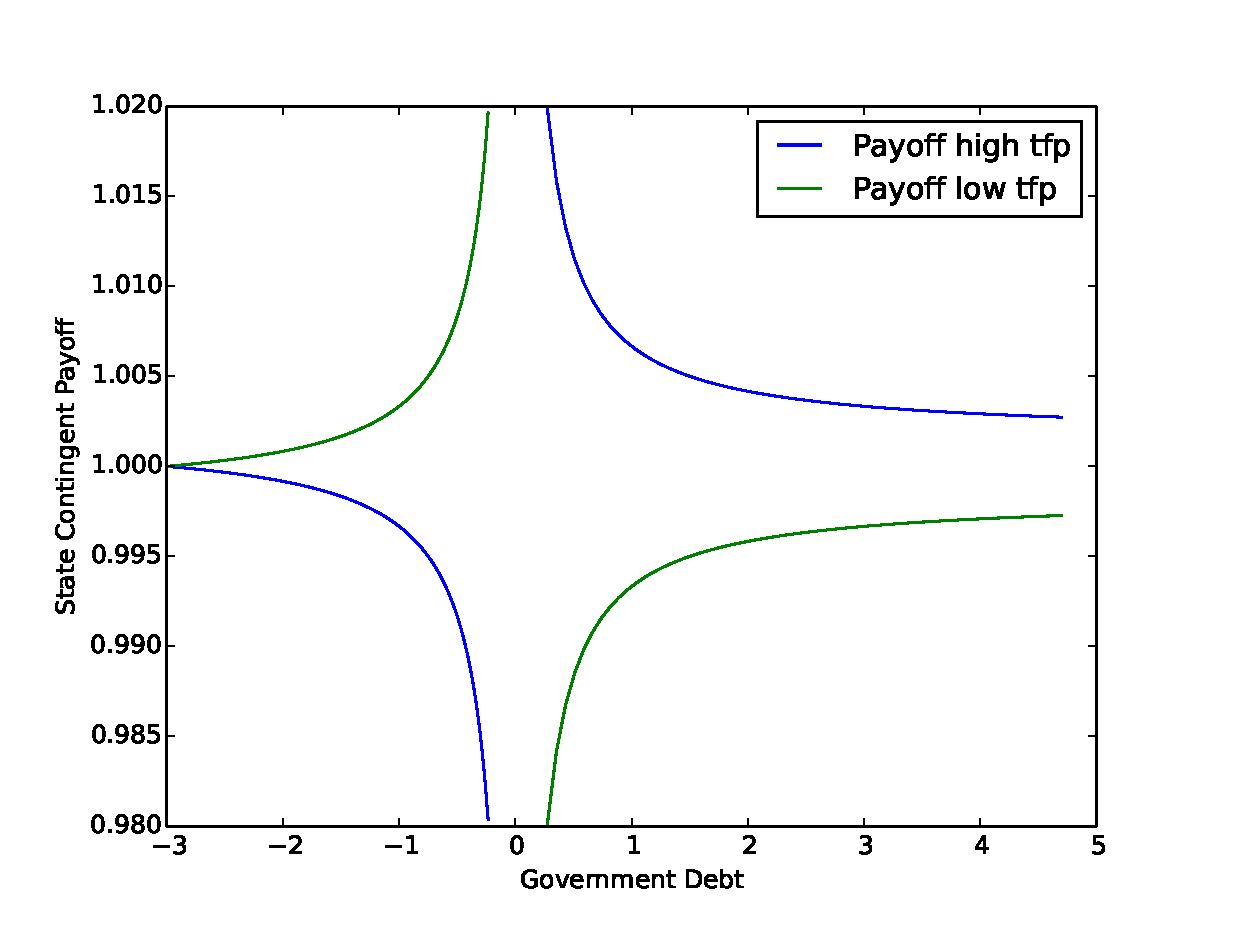
\includegraphics[scale=.4]{Images/p_graph_tfp.eps}
		\caption{Optimal asset payoff structure as a function of initial government debt when TFP follows a 2 shock i.i.d process}
	\end{center}	
	\end{figure}

  \end{frame}

% 
  \begin{frame}
   \frametitle{Optimal Payoff Structure: Expenditure shocks}
	\begin{figure}
		\begin{center}
		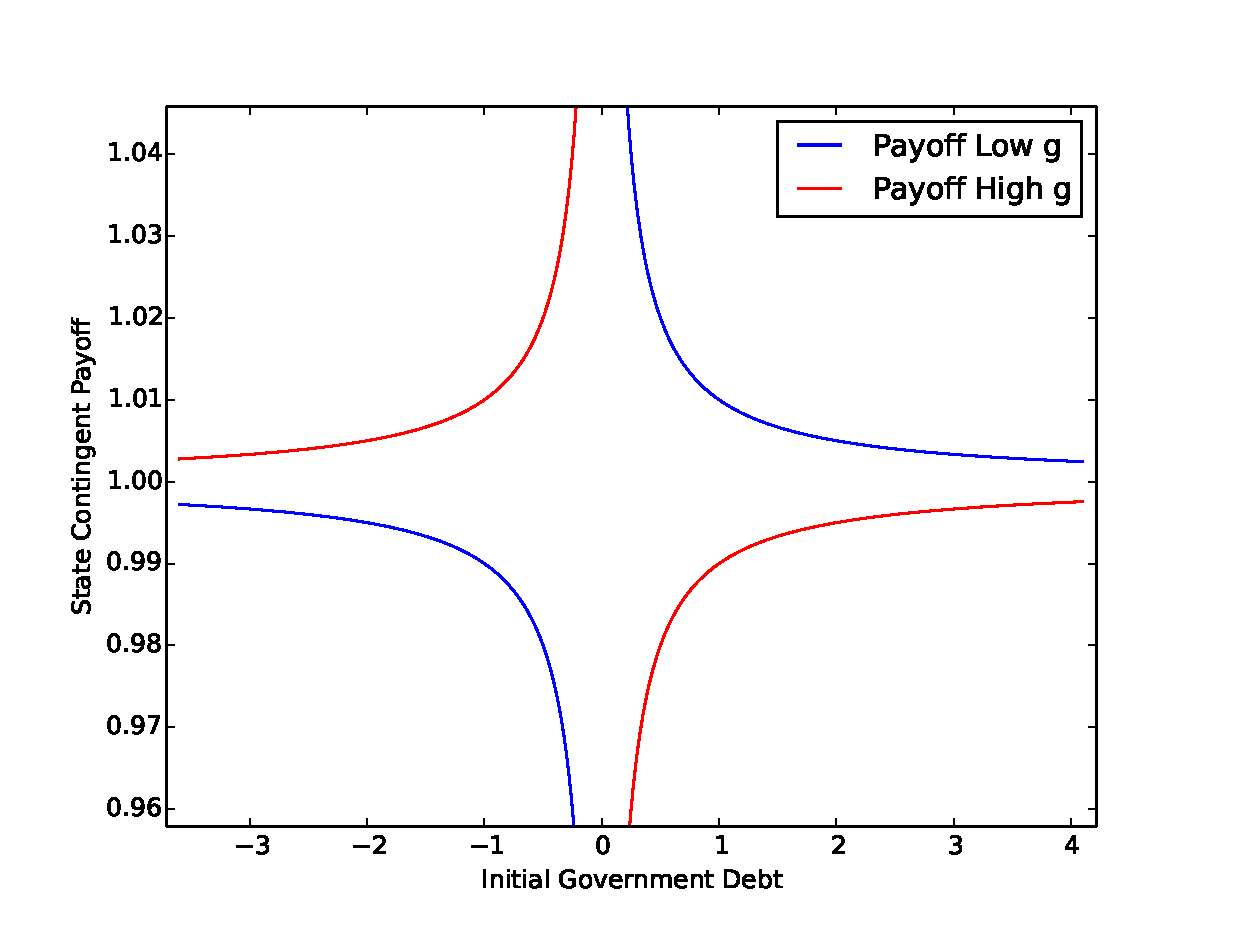
\includegraphics[scale=.4]{Images/p_graph.eps}
		\caption{Optimal asset payoff structure as a function of initial government debt when government expenditures follow 2 shock i.i.d process}
	\end{center}	
	\end{figure}

  \end{frame}
% 
% 

\begin{frame}
   \frametitle{show $b\to b^*$ }
	\begin{figure}
		\begin{center}
		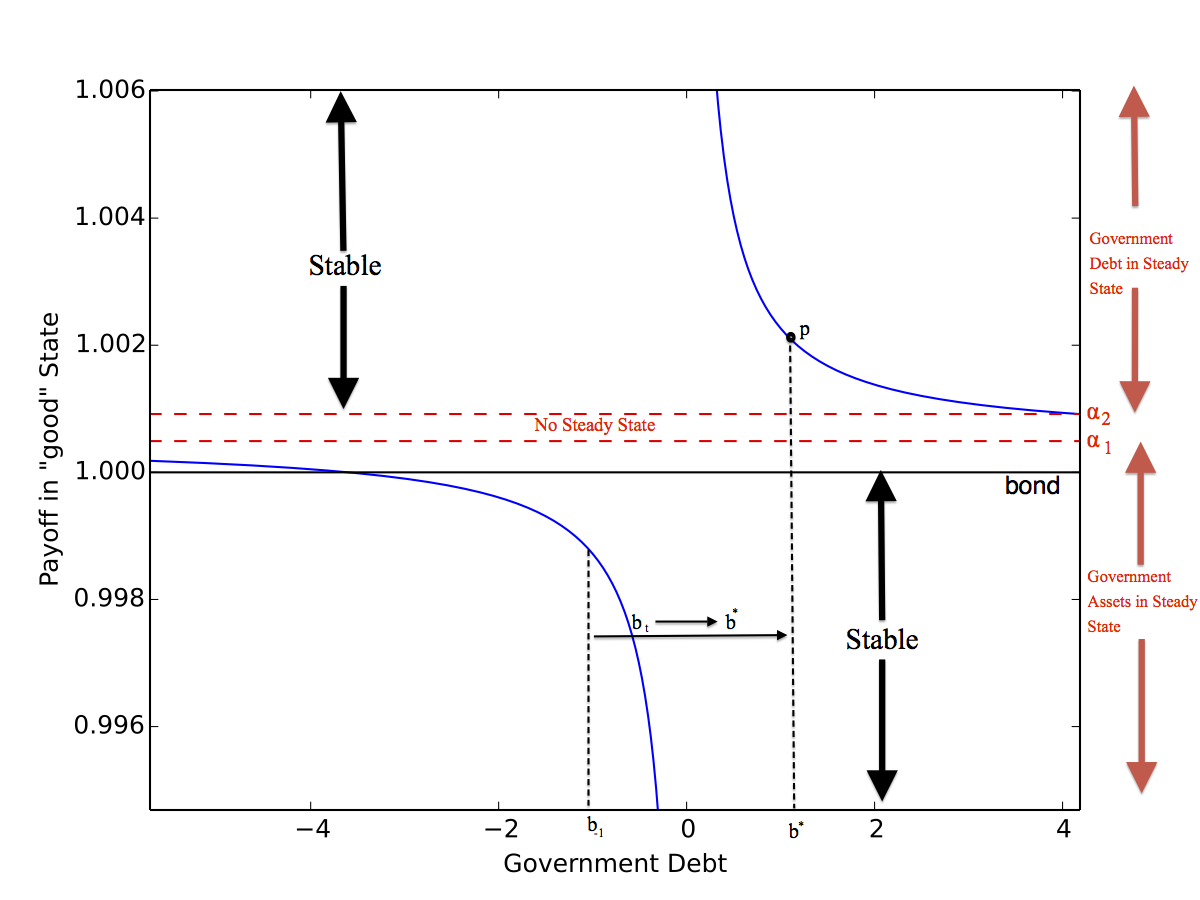
\includegraphics[scale=.5]{Images/graph.png}
	\end{center}	
	\end{figure}

  \end{frame}
 
% 
\begin{frame}
	\frametitle{Incomplete markets }
	\begin{enumerate}
		\item  \textbf{Exogenous payoff structure:} Suppose $\mathbb{P}\neq \mathbb{P}^*(b_{-1})$
		
		\item \textbf{Steady States: } A steady state is a debt level for the government $b^*$ such that 
		\[b_{t}=b^* \text{ implies } b_{t+s}=b^*\quad s>0\]
	
			
		\item \textbf{Characterization: } Given an asset payoff structure $\mathbb{P}$
		\begin{itemize}
			\item Does a steady state exist? is it unique?
			\item What is the level of government debt or   assets in a steady state?
			\item For what levels of  \emph{initial government debt} does  convergence to a steady state occur?
 			\end{itemize}
	\end{enumerate}
\end{frame}



 \begin{frame}
  \frametitle{Existence}
 A steady state is obtained by inverting the optimal payoff structure i.e 
\begin{equation}
\label{eq-ss}
b^*: \mathbb{P}(b^*)=\mathbb{P}^*(b^*)
\end{equation}

 
 When shocks are i.i.d and take two values
 
  \begin{enumerate}
 
\item $\mathbb{P}(s|s\_)$ is independent of $s\_$ 
\item We can normalize $\mathbb{E}\mathbb{P}(s)=1$ and w.l.o.g, denote payoffs by a scalar $\bm{p}$.
\begin{itemize}
 \item $\bm{p}$ is the payoff in the ``good'' state $s$
 \item A risk free bond is a security when $\bm{p}=1$
\end{itemize}
\item  The steady restriction (\ref{eq-ss}) solves one equation in one unknown.  
\end{enumerate}
\end{frame}



\begin{frame}
\frametitle{Existence: Regions in $\bm{p}$ space}
 
The payoff $\bm{p}$ in good state 
$\in (0,\infty)$.

We can decompose a class of economies with different payoff structuresinto 3 regions using thresholds $\alpha_2\geq\alpha_1\geq1$
 
 
 
  \begin{itemize}
   \item Low enough $\bm{p}(\leq \alpha_1$): government holds assets in steady state
   \item High enough $\bm{p} (\geq \alpha_2$): government  issues debt  in steady state
   \item Intermediate $\bm{p} (\alpha_1>\bm{p}>\alpha_2$): steady states do not exist
  \end{itemize}
 
 \end{frame}
% 
\begin{frame}
 \frametitle{Thresholds: $\alpha_1 <\alpha_2$}
	%For either a pure TFP shock or a pure government expenditure shock,  we compute % $\alpha_1$ and $\alpha_2$ directly
	\begin{itemize}
		\item With only government expenditure shocks
		\[
			\alpha_1 = 1 \text{  and }  \alpha_2 = (1-\beta)\frac{\theta^\frac{\gamma}{1+\gamma}\left(\frac{1}{1+\gamma}\right)^\frac1\gamma\frac{\gamma}{1+\gamma}-g(s_1)}{\theta^\frac{\gamma}{1+\gamma}\left(\frac{1}{1+\gamma}\right)^\frac1\gamma\frac{\gamma}{1+\gamma}-\EE g} +\beta>1
		\]
		\item With only TFP shocks
		\[
			\alpha_1 = (1-\beta)\frac{\theta(s_1)^\frac{\gamma}{1+\gamma}}{\EE\theta^\frac{\gamma}{1+\gamma}}+\beta > 1
		\]and
		\[
		\alpha_2 = (1-\beta)\frac{\theta(s_1)^\frac{\gamma}{1+\gamma}\left(\frac{1}{1+\gamma}\right)^\frac1\gamma\frac{\gamma}{1+\gamma}-g}{\EE\theta^\frac{\gamma}{1+\gamma}\left(\frac{1}{1+\gamma}\right)^\frac1\gamma\frac{\gamma}{1+\gamma}-g}+\beta>\alpha_1
		\]
	\end{itemize}
 \end{frame}


\begin{frame}
   \frametitle{show the existence region}
	\begin{figure}
		\begin{center}
		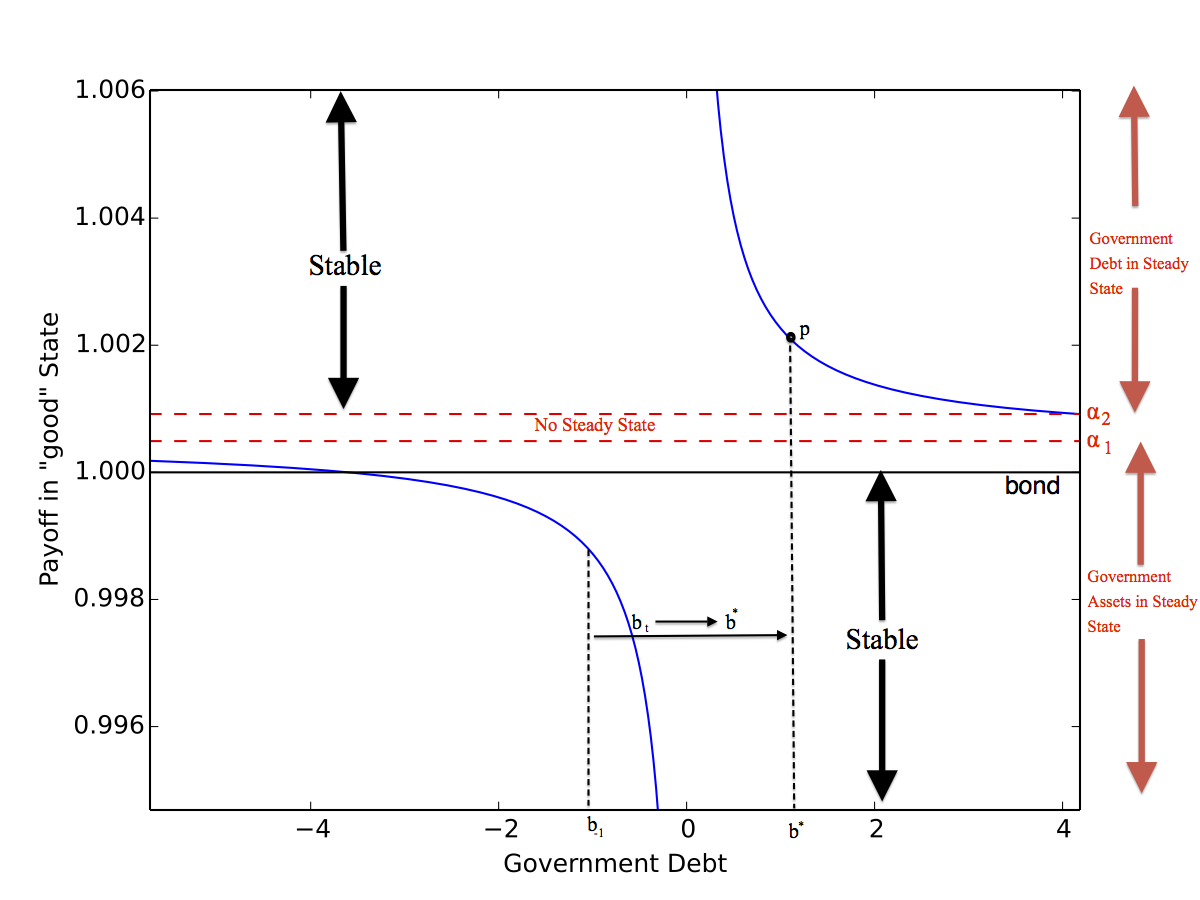
\includegraphics[scale=.5]{Images/graph.png}
	\end{center}	
	\end{figure}

  \end{frame}

  
 \begin{frame}
  \frametitle{Convergence}
  \begin{itemize}
		\item Our analysis verifies the existence of a steady state in a 2-state i.i.d. economy.
		\item To study long-run properties of a Ramsey allocation with incomplete markets, we need to determine whether these steady states are stable
		\item \textbf{Risk-adjusted martingale:}
		
		Under an optimal policy, the Lagrange multiplier $\mu_t$ on the implementability  constraint   satisfies
		\[
			\mu_t = \EE_t p_{t+1} \mu_{t+1}
		\] or
		\[
		\EE_t  \mu_{t+1}	= \mu_t -Cov_t (p_{t+1}, \mu_{t+1})
		\]
			\emph{$\mu_t$ follows a risk adjusted martingale.}
	
		\item \textbf{Stability: }   Away from a steady state, is the drift  $\mu_t$ big enough?
		\end{itemize}
	
 \end{frame}

% 
% 
 \begin{frame}
  \frametitle{Characterizing Convergence}

  \begin{itemize}
  \item Reminder:  $\bm{p}$ is the payoff in the ``good'' state.
   \item As with existence, we can partition  the ``$\bm{p}$ space'' into stable and unstable regions
   
  \end{itemize}
  
  
  
  \end{frame}
  
  \begin{frame}
  \frametitle{}
  
  \small
 	\begin{theorem}
Let $b^*$ denote the steady state level of debt.  Then for  same $  \alpha_1 < \alpha_2$
		\begin{enumerate}
			\item  \textbf{Low $p_1$}: If $p_1\leq\min(\alpha_1,1)$ then the steady state is stable with $b_{fb}<b^*<0$ and $b_t\rightarrow b^*$ with probability 1.
			\item \textbf{High  $p_1$}:  If $p_1 \geq \alpha_2$ then the steady state is stable with $0<b^*$ and $b_t \rightarrow b^*$ with probability 1.
			
			
			\end{enumerate}
			\end{theorem}
			
			For the intermediate region where either $b^*$ does not exist or is unstable, there is a tendency towards accumulating debt
		
		
	
 \end{frame}

 
\begin{frame}
   \frametitle{Show the stable region}
	\begin{figure}
		\begin{center}
		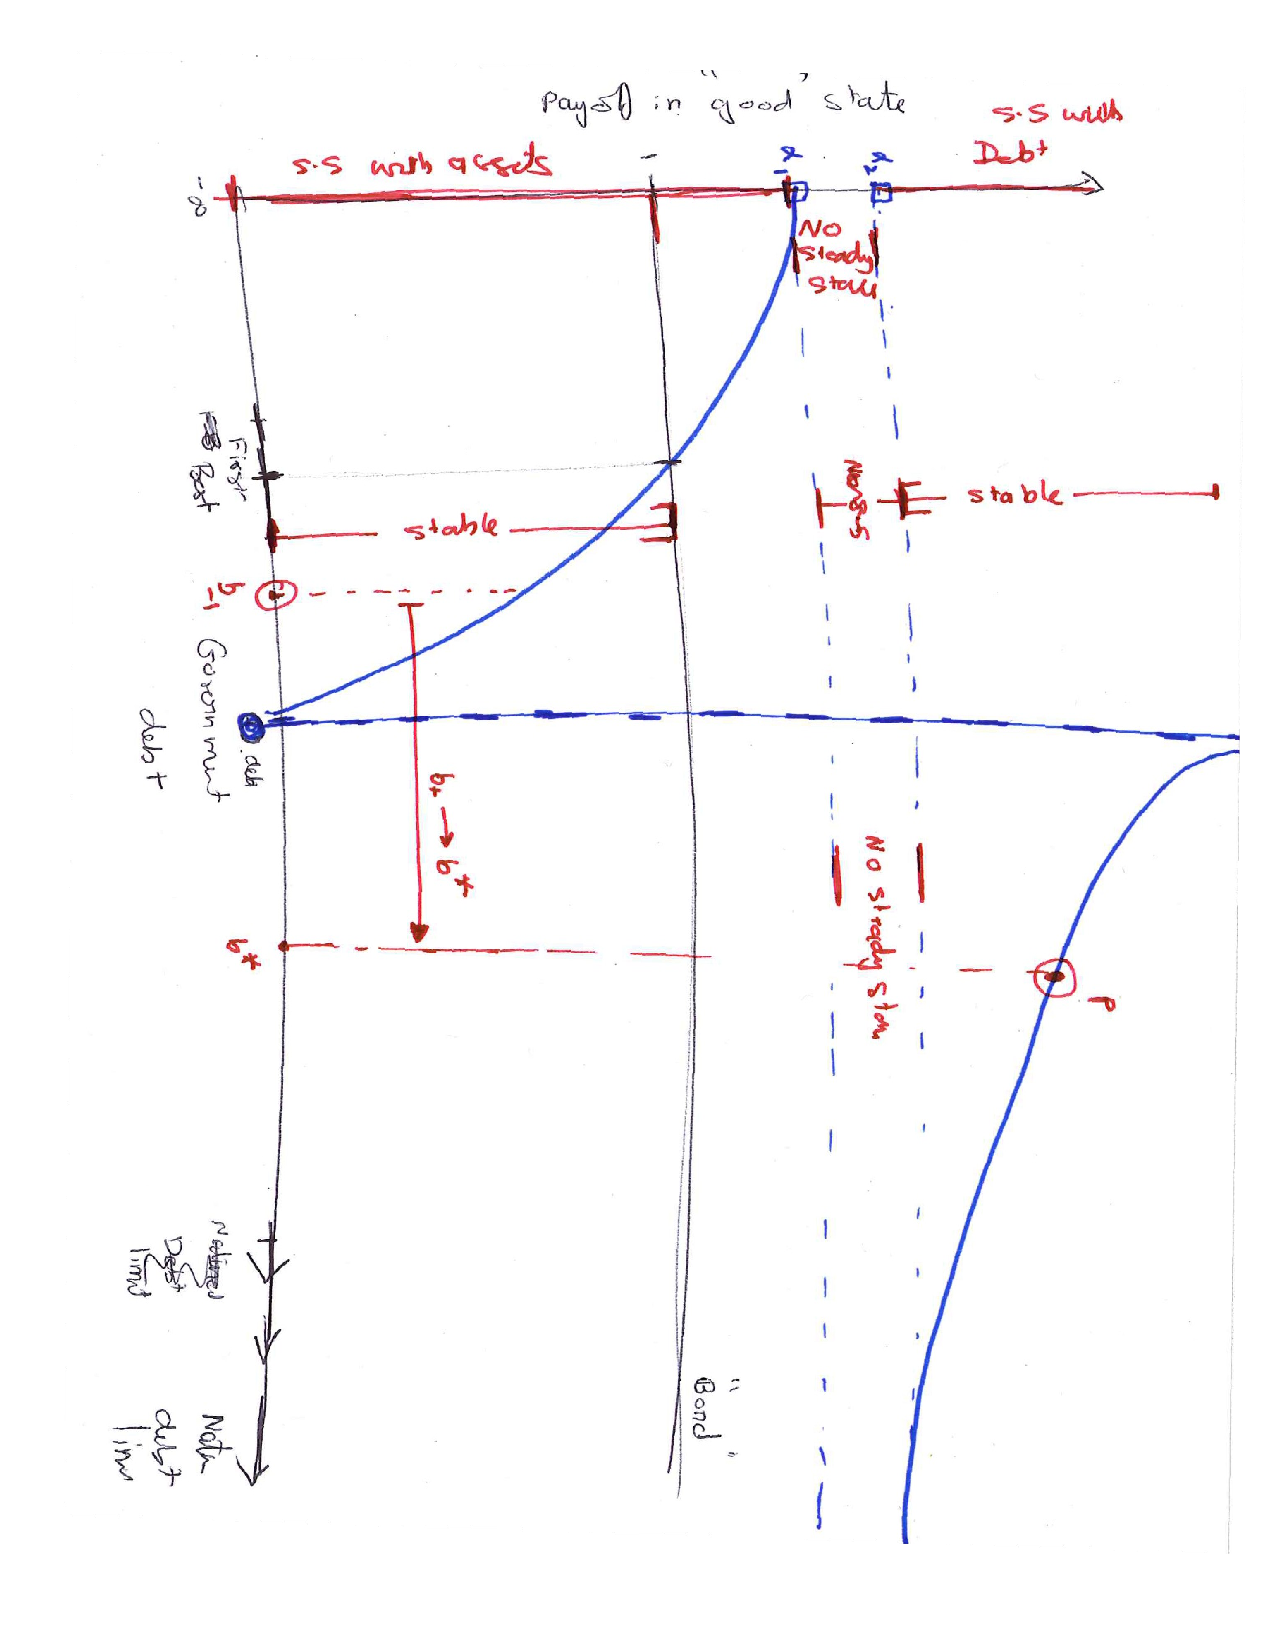
\includegraphics[scale=.3,angle=90]{Images/tempGraph.pdf}
	\end{center}	
	\end{figure}

  \end{frame}

 
 \begin{frame}

	\frametitle{$p_1 > 1$}
	\begin{center}
	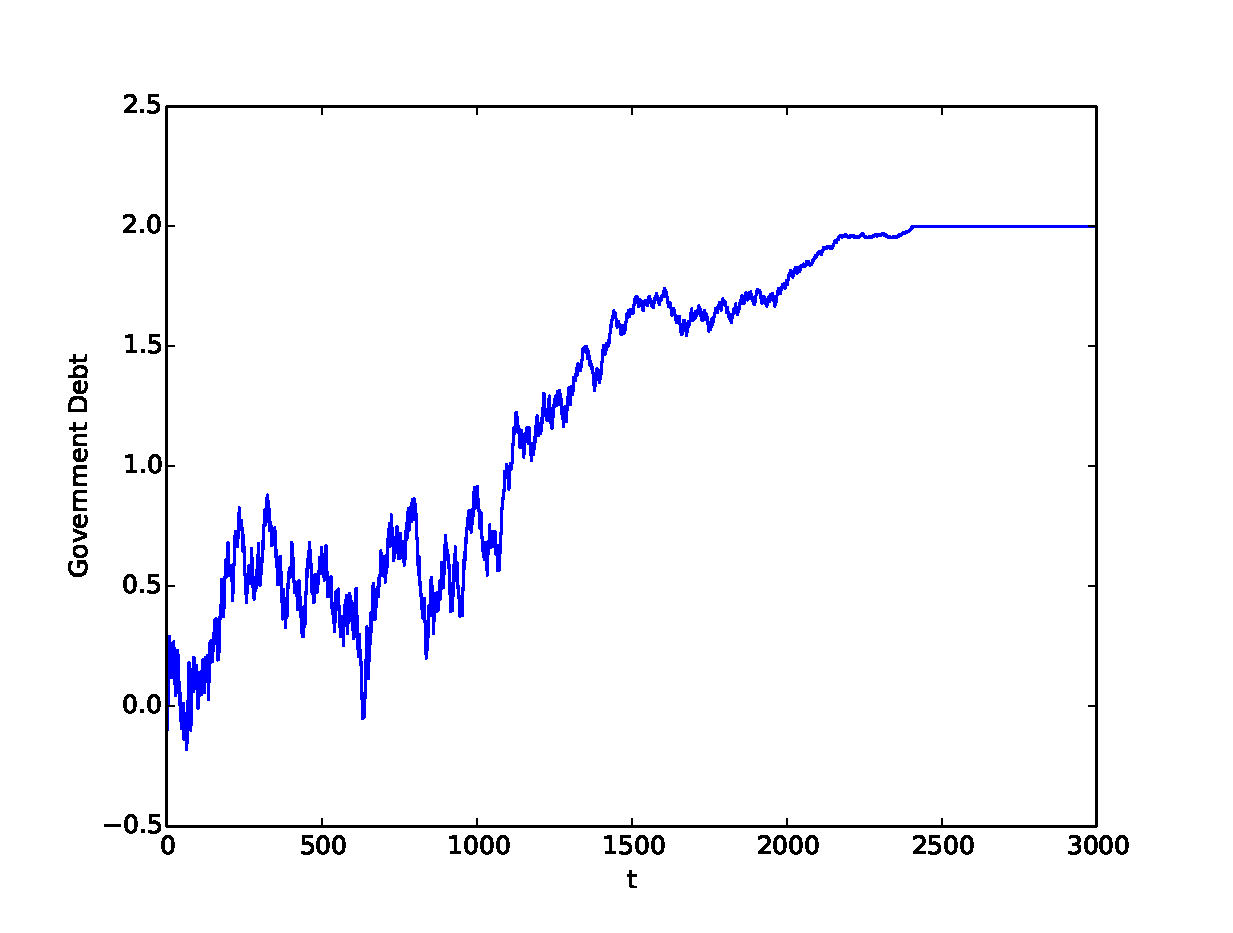
\includegraphics[width=4in]{Images/port1.eps}
	\end{center}
\end{frame}

\begin{frame}
	\frametitle{$p_1 < 1$}
	\begin{center}
	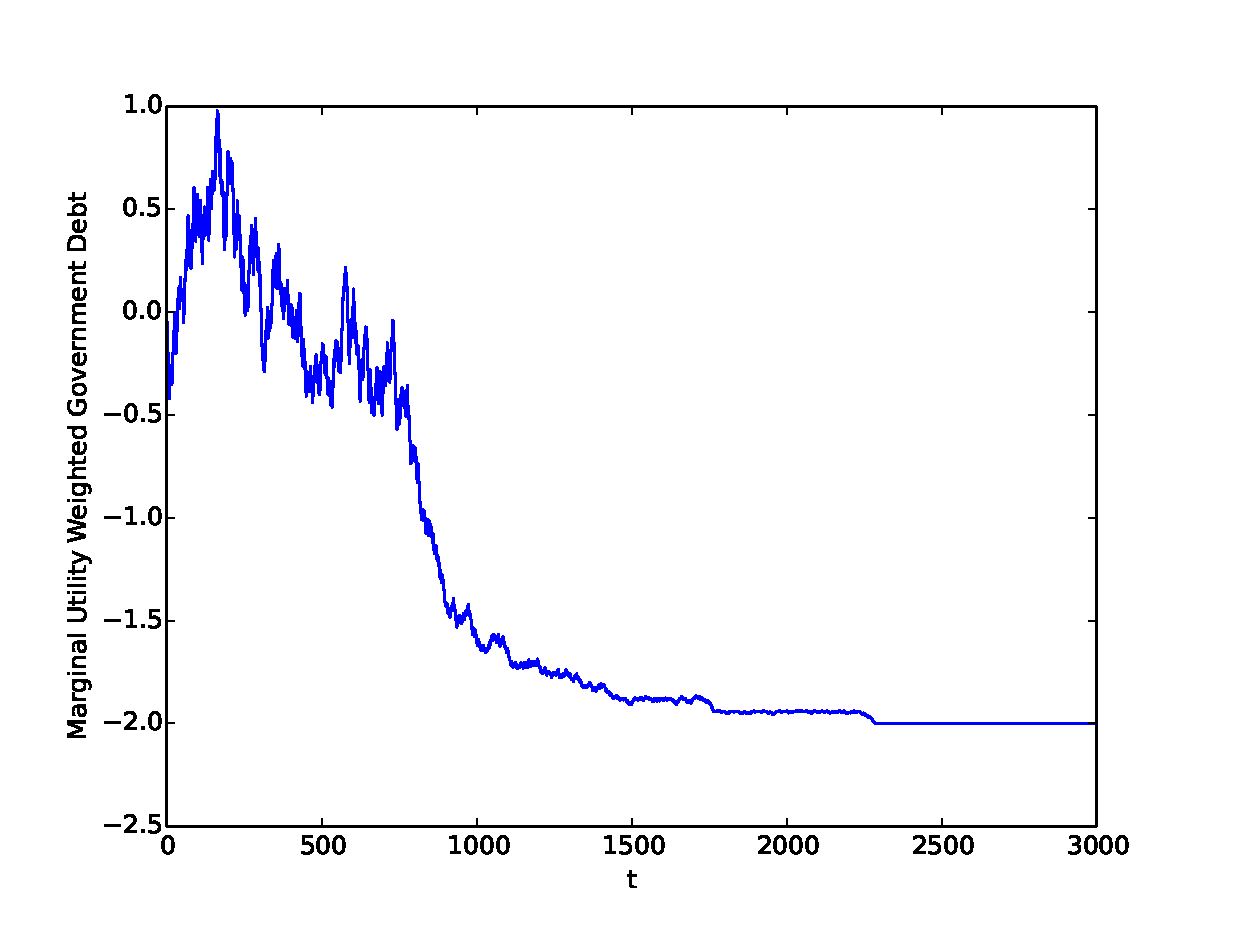
\includegraphics[width=4in]{Images/port2.eps}
	\end{center}
\end{frame}
%
% \begin{frame}
% 	\frametitle{Intuition and Generalizations}
% 	\begin{enumerate}
% 		\item The intuition we gain from our 2-state example is that, given exogenous payoff restrictions on government debt, there exist debt positions that allow the government to better smooth tax distortions across states.
% 		\item  Over time, the government adjusts it's debt position in order to best reallocate resources across states.
% 		\item  \textbf{Extensions: } more general preferences and more general aggregate state processes.
% 		\begin{itemize}
%
% 		\item  With risk aversion we are able to obtain similar results under the 2 state i.i.d assumption.
% 		\item More general processes require us to develop computational tools to analyze the long run dynamics
% 		\end{itemize}
%
% 		%\item  For more general aggregate state processes there no longer exists a complete markets %steady state.
% 		%\item  This requires us to develop computational tools to analyze the long-run dynamics.
% 		%\item  We find that with more general processes there exist regions with low volatility, because the government's debt position is reallocating resources across states and in the long run the government debt converges to these regions.
% 	\end{enumerate}
% \end{frame}
% %
\begin{frame}
 \frametitle{Incomplete markets with risk aversion}
 \textbf{Quasilinear preferences: }
 \begin{enumerate}
  \item With quasilinear preferences, we showed that $b_t\to b^*$ when the aggregate state follows a 2-state i.i.d. process
  \item The level  and sign of $b^*$ is a function of the \textbf{exogenous payoff structure} $\mathbb{P}$
  \item The limiting allocation corresponds to a complete market allocation
 \end{enumerate}

 \textbf{Risk aversion:}
  \begin{itemize}
   \item This marginal utility adjusted debt will encode history dependence
   \item Instead of government debt  $x_t=u_{c,t}b_{t}$ will converge with binary i.i.d shock shock process

   \item Long-run properties of $x_t$ depend on returns $R_{t,t+1}=\frac{\mathbb{P}(s_{t+1}|s_t)}{q_t(s^t)}$

  \end{itemize}
  %\emph{To retain analytical tractability and clarify our analysis we will remove exogenous fluctuations in the payoff terms by restricting $p(s) =1$}
  \end{frame}
%
\begin{frame}
\frametitle{Roadmap, II}
\begin{itemize}

\item Split the Ramsey problem in two
\begin{enumerate}
 \item  $t=0$ Bellman equation in $W(b_{-1},s_0)$ %\textcolor{red}{Anmol and David XXXXXX: I altered the notation}
 \item  $t\geq 1$ Bellman equation in $V(x,s\_)$
\end{enumerate}

\item Analyze steady states $x^*$ such that $x_t \to x^*$

\end{itemize}
So far,
\begin{enumerate}
 \item \textbf{Risk free bond} Existence proved only under a special case of a risk-free bond  $\mathbb{P}(s|s\_)=1 \forall s,s\_$ 
 
 This focuses on \textit{endogenous} component of returns

 \item \textbf{Interpretation:}  $x^*$  corresponds to an initial condition when the optimal portfolio in a LS economy is a risk-free bond

\end{enumerate}

\end{frame}


 \begin{frame}
	\frametitle{A Recursive Formulation}
	
	\begin{enumerate}
	 \item Commitment implies that government actions at $t \geq 1$ are constrained by  anticipations about them at $s < t$
	 \item This contributes additional state variables like marginal utility of consumption
	 \item Scaling the budget constraint by marginal utility makes it recursive in  $x=U_c b$
	
	\[
		\frac{x_{t-1} p_t U_{c,t}}{\beta \EE_{t-1} p_t U_{c,t}}  = U_{c,t}c_t+U_{l,t} l_t + x_t
	\]
	
	%\item The planner's problem recursively with a single state variable.
	\end{enumerate}
	
	
	\end{frame}
	\begin{frame}
	\frametitle{Bellman equation for $t\geq1$}
	\[
		V(x,s\_) = \max_{c(s),l(s),x'(s)} \sum_s \pi(s,s\_)\Bigl(U(c(s),l(s)) + \beta V(x'(s),s)\Bigr)
	\]subject to $x'(s)\in [\underline x,\overline x]$
	\begin{align*}
		\frac{x p(s) U_c(s)}{\beta\EE pUc} =U_c(s)c(s)+U_l(s)l(s) + x'(s)\\
		c(s) + g(s) = \theta(s)l(s)
	\end{align*}
	
 \end{frame}
\begin{frame}
	\frametitle{Time $0$ Bellman equation}
	Given an initial  debt $b_{-1}$, state $s_0$,  and continuation value function $V(x,s\_)$
%\textcolor{red}{Anmol and David XXXXX: I altered the below by adding the $W$ function; but there is a problem with the timing of
%the $b$ argument.  See earlier slide where $W$ is defined.}
	\[
		W(b_{-1},s_0) = \max_{c_{0},l_0,x_{0}} U(c,l) +\beta V(x_0,s0)
	\]subject to  time zero implementability constraint
	\[
		U_{c}(c_0,l_0)c + U_l(c_0,l_0) l_0 + x_0 = U_c(c_0,l_0) b_{-1}
	\]and  resource constraint
	\[
		c_0+ g(s_0) = \theta(s_0) l_0
	\]and
	\[
		x_0 \in [\underline x,\overline x]
	\]
\end{frame}



\begin{frame}
 \frametitle{Revisiting steady states with risk aversion}
Let $x'\left( s;{x},s\_\right) $ be an optimal  law of motion for the state variable
for the $t\geq1$ recursive problem.

\begin{definition}
 A steady state  ${x}^{*} $  satisfies ${ x}^{*}  =x' \left( s;{x}^{*},s_{-}\right) $ for all $%
\,s,s\_$
\end{definition}


\vspace{3mm}
\emph{Thus, a steady state is a node at which  continuation allocation and tax rate have no further history dependence. }

 \end{frame}




 \begin{frame}
	\frametitle{Existence}
	
	\begin{enumerate}
	 \item For a class of economies with separable iso-elastic preferences
	 $U(c,l) = \frac{c^{1-\sigma}}{1-\sigma} -\frac{ l^{1+\gamma}}{1+\gamma}$
	 \item Shocks that take two values and are i.i.d
	\end{enumerate}

	
	Let $x_{fb}$ be a value of the state $x$ from which the government can implement first best from that period onwards.  
	
	
	
	
	\begin{proposition}  Let $q^{fb}(s)$ be the shadow price of government debt in state $s$ and using the first best allocation. 
	if 
	\[
		\frac{1-q^{fb}(s_b)}{1-q^{fb}(s_g)} > \frac{g(s_b)}{g(s_g) }
	\] 
	
	Then there exists a steady state with $x^{fb}>x^*>0$
		\end{proposition}
\end{frame}


%



%
%
%
% \begin{frame}
% 	\frametitle{A Recursive Approach: Time 0}
% 	Given the initial debt level $b_0$, state $s_0$,  and the continuation value function $V(x,s\_)$ the planner's problem is then to solve the following
% 	\[
% 		\max_{c,l,x'} U(c,l) +\beta V(x',s0)
% 	\]subject to the time zero implementability constraint
% 	\[
% 		U_{c}(c,l)c + U_l(c,l) l + x' \geq U_c(c,l) b_0
% 	\]and the resource constraint
% 	\[
% 		c+ g(s_0) = \theta l
% 	\]and
% 	\[
% 		x' \in [\underline x,\overline x]
% 	\]
% \end{frame}
%
%
% %
% %   \item With risk aversion
% %   \item  To clarify our analysis we will remove exogenous fluctuations in the payoff terms $p_t U_{c,t}$ by restricting $p_t =1$.
% %  \end{enumerate}
% %
% % 	      \item quasilinear analysis found that there existed steady states when the aggregate state followed a 2 -state i.i.d. process.
% % 		\item Marginal utility weighted debt $x_t b_t U_{c,t}$ indexes the the space of optimal allocations with state contingent debt
% % 		\item  We would therefore expect a steady states to exist for the variable $x$
% % 		\item  To clarify our analysis we will remove exogenous fluctuations in the payoff terms $p_t U_{c,t}$ by restricting $p_t =1$.
% % 		\begin{itemize}
% % 			\item  Note under this restriction the endogenous payoff terms will be larger in bad states of the world, and thus, the government will hold assets in the steady state
% % 		\end{itemize}
% % 	\end{itemize}
% %\end{frame}
%
%
% \begin{frame}
% 	\frametitle{Incomplete Market's with Risk Aversion}
% 	\begin{itemize}
% 	\item By choosing a new variable $x_{t-1} = b_{t-1} U_{c,t-1}$ the measurability constraints can be written as a period by period constraint
% 	\[
% 		\frac{x_{t-1} p_t U_{c,t}}{\beta \EE_{t-1} p_t U_{c,t}}  = U_{c,t}c_t+U_{l,t} l_t + x_t
% 	\]
% 	\item  This bares a striking resemblance to the period by period constraint for quasi-linear preferences
% 	\[
% 		\frac{b_{t-1} p_t}{\beta \EE_{t-1} p_t} = c_t + U_{l,t} l_t + b_t
% 	\]
% 	\item  The $p_tU_{c,t}$ terms in the risk averse budget constraint act as endogenous payoffs.
% 	\end{itemize}
% \end{frame}
%
%  \begin{frame}
% 	\frametitle{Existence}
% 	Let $x_{fb}$ be the $x$ with which the government can institute first best from that period onwards.  Assume a CRRA utility specification $U(c,l) = \frac{c^{1-\sigma}}{1-\sigma} -\frac{ l^{1+\gamma}}{1+\gamma}$.  Finally, let  $c^{fb}$ and $l^{fb}$ be consumption and leisure under first best.  We have the following proposition
% 	\begin{proposition}  For a 2 state i.i.d. process let  $s_g$ and $s_b$ denoting the states with high and low consumption at first best.  If
% 	\[
% 		\frac{g(s_g)}{1-\frac{\beta\EE[(c^{fb})^{-\sigma}]}{c^{fb}(s_g)}} > \frac{g(s_b)}{1-\frac{\beta\EE[(c^{fb})^{-\sigma}]}{c^{fb}(s_b)}}
% 	\]  Then there exists a multiplier $\mu$ and complete markets solutions $c^\mu,l^\mu$ such that
% 	\[
% 	\underline x<\frac{U_{c_\mu}(s)c_\mu(s) + U_{l_\mu}(s) l_\mu(s)}{\frac{U_{c_\mu}(s)}{\beta\EE[U_{c_\mu}]}-1} = x^* <0
% 	\]
% 	\end{proposition}
% \end{frame}
%
%
\begin{frame}
	\frametitle{Stability}
	\begin{enumerate}
	 \item In this setup, interest rates are aligned with marginal utility of consumption;  they are low  in ``good'' states (high TFP or low expenditure)
	 \item The government holds claims against the private sector in the steady state. This is similar to the quasilinear case when $p_1$ was low.	 
	 \item The incomplete markets Ramsey allocation converges to a Lucas-Stokey  Ramsey allocation for all initial conditions	 	
	\end{enumerate}


	\begin{proposition}  Let $\{c_t(s^t), l_t(s^t), x_t(s^{t-1})\}$ solve the incomplete markets Ramsey problem.  Then  $x_t(s^{t-1})\rightarrow x^*$ as $t\rightarrow \infty$ with probability 1 for all initial conditions
	
	\end{proposition}
	\end{frame}
	
%
\begin{frame}
	\frametitle{Quasilinear vs. risk aversion}
	{\color{red} Redo this slide}
	\begin{itemize}
				\item  With  quasilinear preferences and a risk-free bond, the interest rate is always $1/\beta$.
   \item With risk averse preferences, interest rate is higher in periods of high government expenditure.
		\item  Thus, while the government has greater expenses in high government expenditure states, the higher interest rate means that the government can  accumulate less and still  cover future government expenditures.
		\item  After the government has accumulated enough assets, it is actually better off in periods of high government expenditure than in periods with low government expenditures (since its claims to consumption are worth more).
		\item  By holding assets, the government is able to reallocate resources across states, something it is not able to do in the quasilinear case.
	\end{itemize}
\end{frame}

\begin{frame}
	\frametitle{2 State i.i.d. process with Risk Aversion}
	\begin{center}
	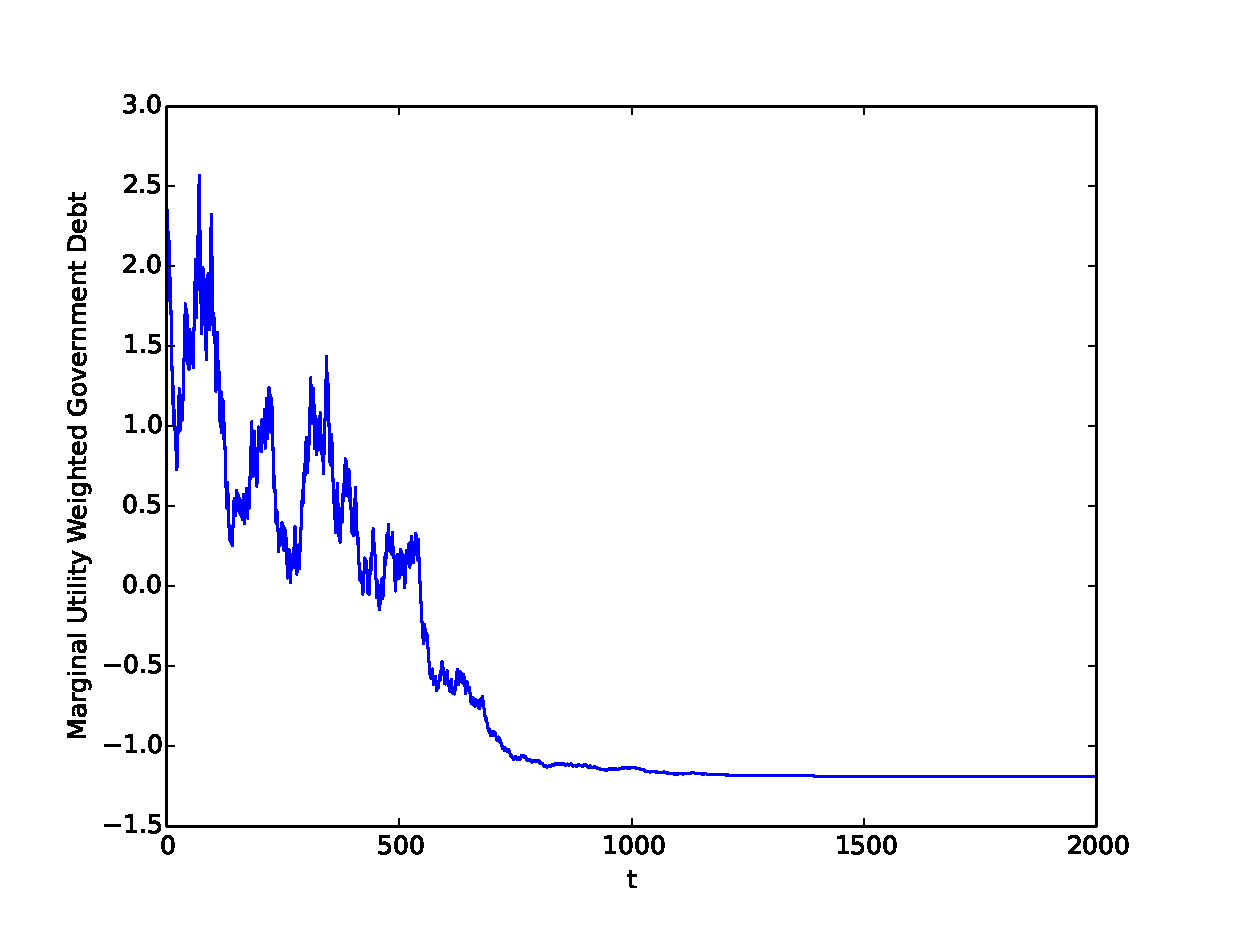
\includegraphics[width=4in]{Images/2stateiid.eps}
	\end{center}
\end{frame}

\section{Numerical Results}
\subsection{}

\begin{frame}
	\frametitle{$S>2$ states}
	\begin{center}
	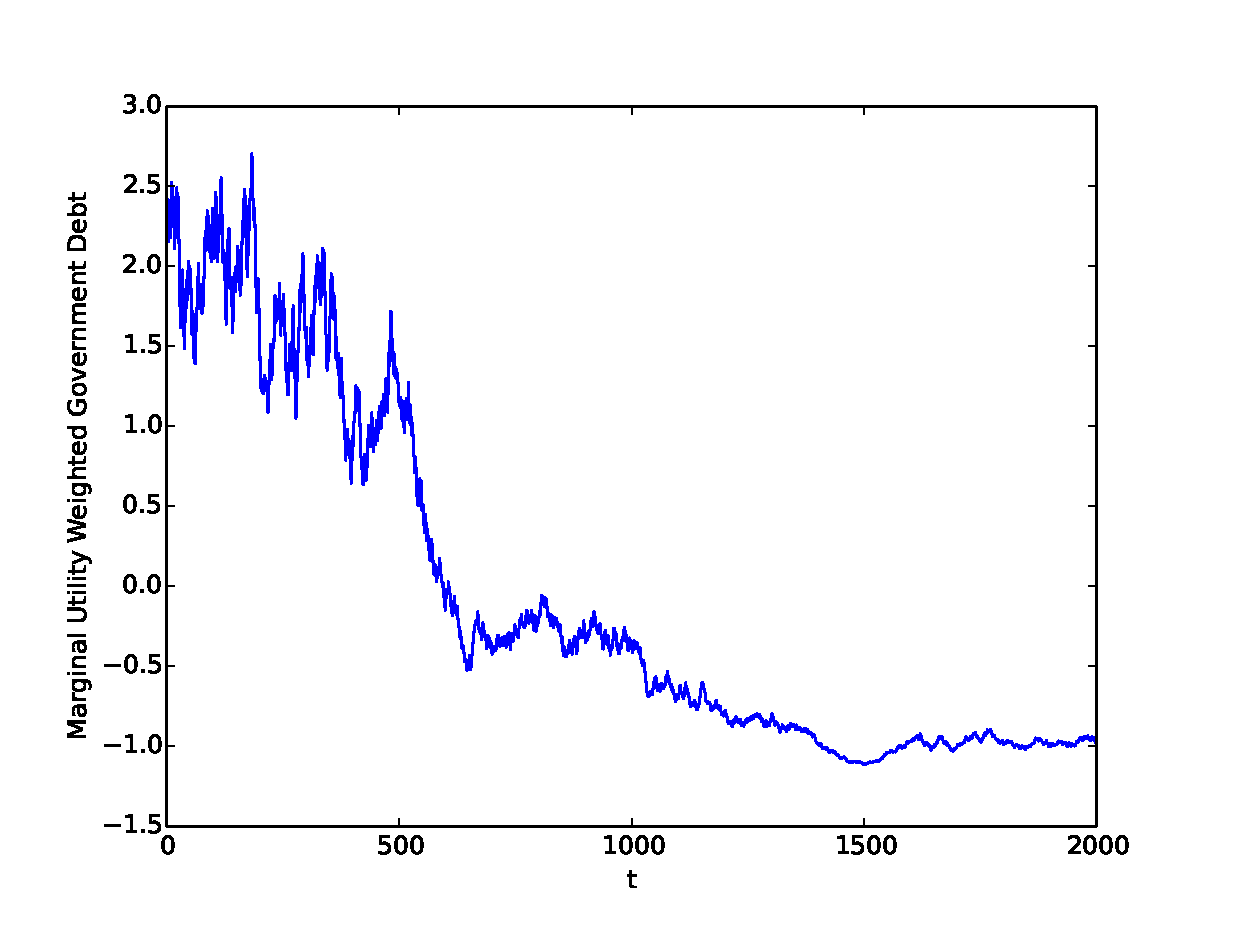
\includegraphics[width=4in]{Images/5stateiid.eps}
	\end{center}
\end{frame}



 \begin{frame}
  \frametitle{Transfers}
	\begin{itemize}
	\item  That the government can use its assets to smooth tax rate distortions carries over to when the government has access to lump sum transfers
	\item Access to nonnegative transfers makes first-best level of assets trivially a ``steady state''.    	
\item  With lump sum transfers,  in cases where the steady state exists and is stable, if the initial debt of the government exceeds its steady state,  the economy  converges with probability 1 to the steady state.
		
	\end{itemize}
 \end{frame}

 \begin{frame}
	\frametitle{Quasilinear preferences and risk-free bond  with and without transfers}
	\begin{center}
	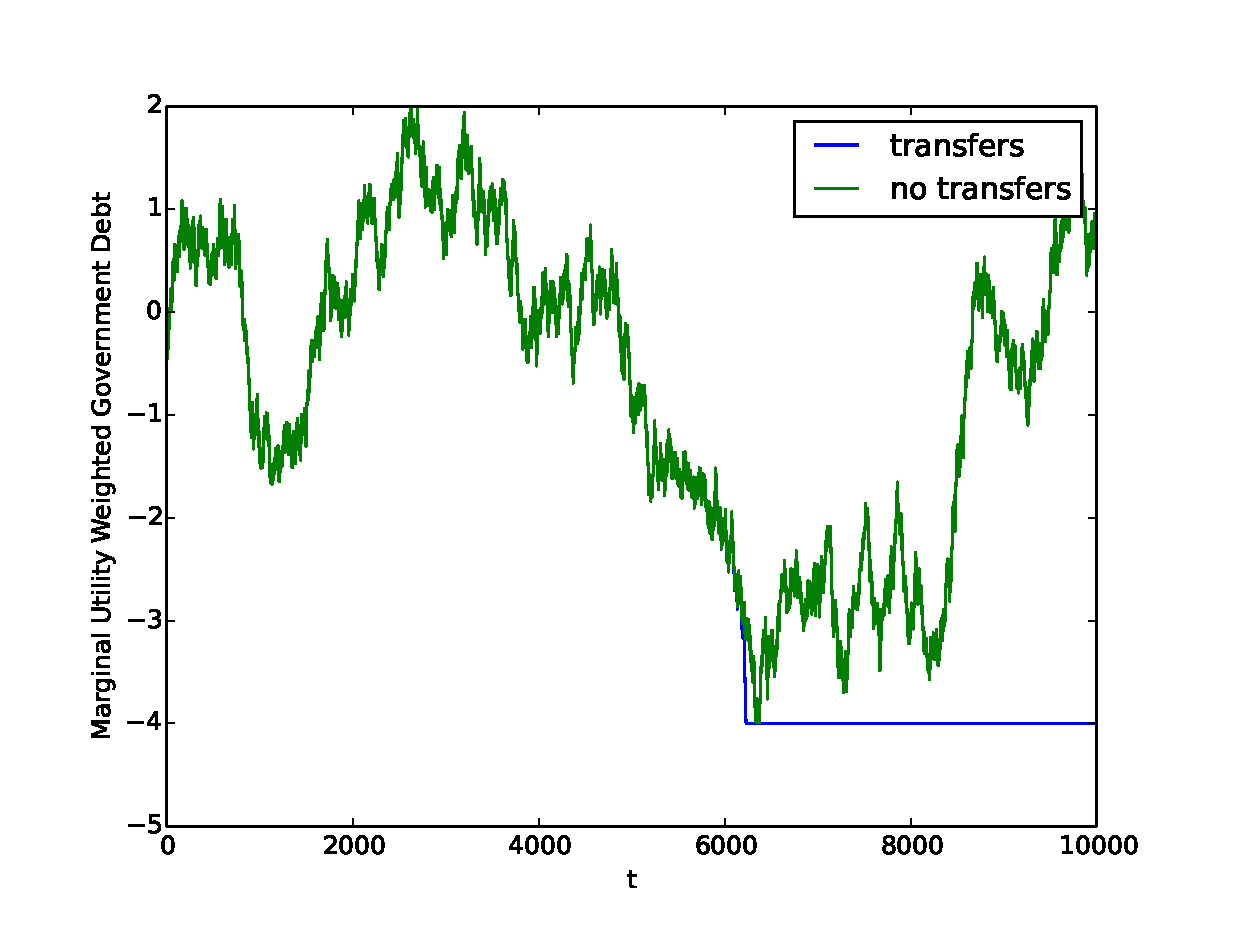
\includegraphics[width=4in]{Images/transfer_example2.eps}
	\end{center}
\end{frame}

\begin{frame}
 Add a slide comparing stuff to Buera Nicolini, Angelotos
\end{frame}

 \begin{frame}
  \frametitle{Concluding remarks }
\begin{itemize}
	\item With market incompleteness, the asset payoff structure  has big implications a Ramsey government's  long run debt
	\item If the asset offers lower returns in adverse states of the world, the Ramsey government  asymptotically runs up a  debt to the private sector.
\item With risk aversion, cyclical properties of interest rate affects government debt asymptotically
	\item  Access to nonnegative transfers play little role in shaping outcomes.  Rather, the key  force is the government's ability to use its debt position to reallocate resources across states
	\item  \textbf{Future Research}:   With heterogeneous agents and unrestricted transfers, how does the type of market incompleteness affect long run wealth distributions and other outcomes?
\end{itemize}
 \end{frame}

  \end{document}
%  